\assignementTitle{Выбор участка территории}{35}{}

\begin{itemize} 
    \item Выберите участок территории города и объекты для реализации тематической экскурсии. Предоставьте выбранный участок территории в виде карты-картинки, соотношение сторон которой примерно равно золотому сечению. 
    \item Обоснуйте свой выбор в текстовой форме, 1-3 предложений. На выбранном участке территории определите объекты интереса - достопримечательности, не менее 10 мест-локаций. Соберите первичную информацию о их расположении и о том, как они выглядят (фото объектов).
    \item Определить гео-координаты каждой достопримечательности.
    \item На выбранный участок карты нужно нанести клеточные поля разных размеров для получения отображения участка территории с высоким (сильно детализированным), средним и низким (один квадрат = 1 объекту достопримечательности - архитектурного сооружения) разрешением. На поле отметить положение выбранных достопримечательностей. 
    \item Выписать координаты объектов  (x,y), сопоставить их с гео-локационными (lat,long). 
    \item Составить JSON по шаблону, представленному на рисунке 1.1.
    
    \putImgWOCaption{14cm}{json}
    \begin{center}
        Рис.1.1. Шаблон JSON для представления данных о POIs тематической экскурсии
    \end{center}    
\end{itemize}

\markSection

\begin{enumerate}
    \item Наличие карты-картинки для выбранного участка территории. Отношение длины а к ширине  b выбранного прямоугольного участка карты должно быть примерно равно золотому сечению - 1.618  (3 балла).
    \item Есть краткое обоснование выбранного для экскурсии участка города, 1-3 предложения. Определены не менее 10 объектов (достопримечательностей), есть фотографии с их внешним видом, названия и адреса местонахождения (5 баллов). 
    \item Определены координаты lat, long каждой достопримечательности (6.8 баллов).
    \item Сделано разбиение карты на поля разных размеров для получения отображения участка территории с высоким, средним и низким разрешением (1.7 балла за каждый вариант, 5.1 баллов за все три варианта)
    \item Определены координаты x, y каждой достопримечательности для соответствующего разрешения карты (5.1 баллов)
    \item Координаты x, y валидны. Т.е. координаты lat и lon: правильно переведены в правую систему координат для соответствующего разрешения, JSON по заданному шаблону составлен валидно: JSON-валидатор \url{https://jsonlint.com} ошибок не выдает. (10 баллов).    
\end{enumerate}

* Проверка соответствия решения критериям 4-6 делается по представленным трем вариантам файлов json с  высоким, средним и низким  разрешением представленного участка территории.

Общее количество баллов: 35. 

\solutionSection

После обсуждения командой разработчиков был выбран участок городской территории, представленный картинкой ниже, рис 1.2.  Ширина фрагмента $b=6.5$, $a=10.5$; $a:b=1.615$ - приблизительно соответствует золотому сечению. 

\textit{Оценка - 3 балла}

Проведение тематической экскурсии на данном участке позволит познакомиться с историческим центром Иркутска, погрузиться в атмосферу старого купеческого города, увидеть архитектурные решения разных исторических эпох. 

\putImgWOCaption{14cm}{1}

\begin{center}
    Рис.1.2.  Карта участка территории, выбранного для тематической экскурсии (ширина фрагмента $b=6.5$, $a=10.5$; $a:b=1.615$ -приблизительно соответствует золотому сечению)
\end{center}

На данном участке территории, в качестве точек интереса, определены 10 достопримечательностей, представленных в таблице 1.

\begin{center}
    Таблица 1. Объекты тематической экскурсии по историческому центру города Иркутска
\end{center}

\begin{longtable}{|p{7.5cm}|p{7.5cm}|}
    \hline
    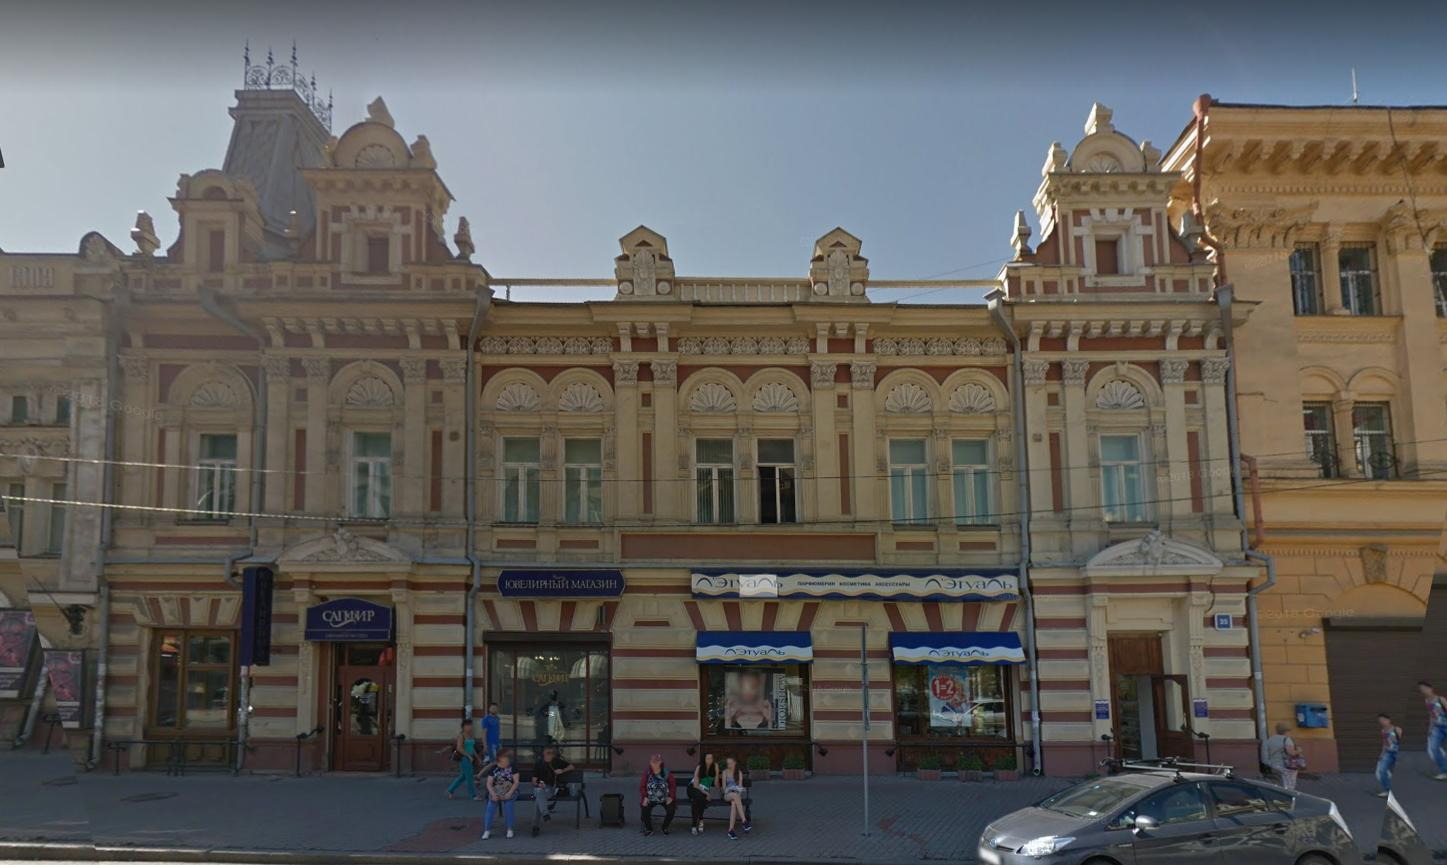
\includegraphics[width=6.5cm]{2} & 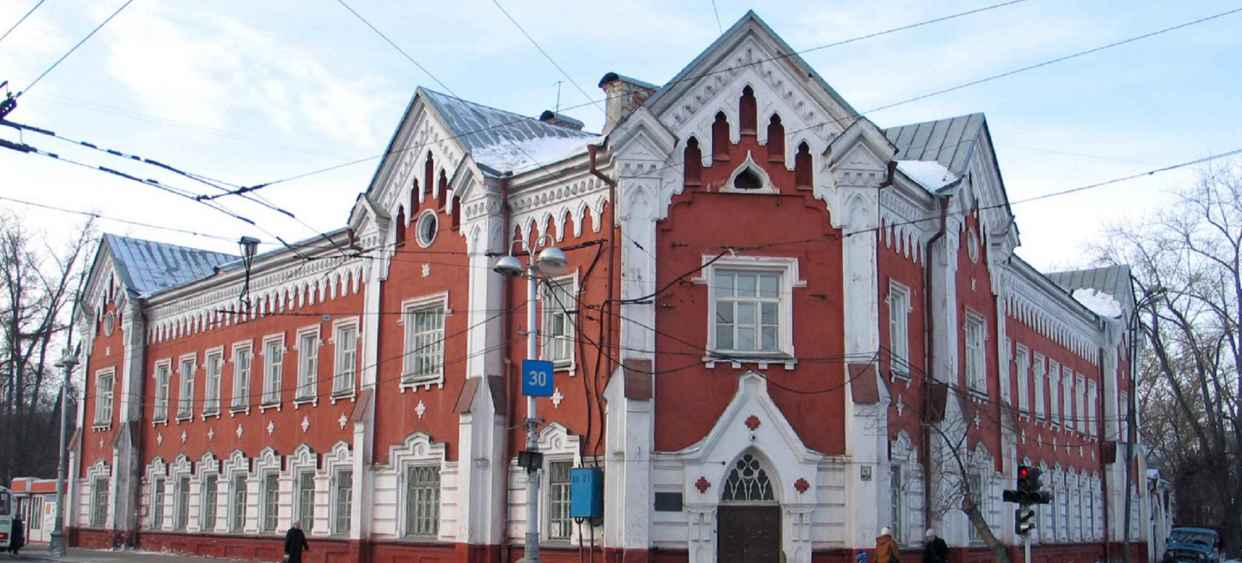
\includegraphics[width=7cm]{3} \\
    \hline
    Дом купца И.И. Базанова  (Гастроном №1)

    Карла Маркса, 25 
    
    52.284283, 104.287344
    
    Ранее: Дом купца И.И. Базанова & Дом Базанова (факультетские клиники ИГМУ) 

    Свердлова, 14 

    52.283765, 104.279034

    Ранее: Базановский воспитательный дом для детей до 1 года \\
    \hline
    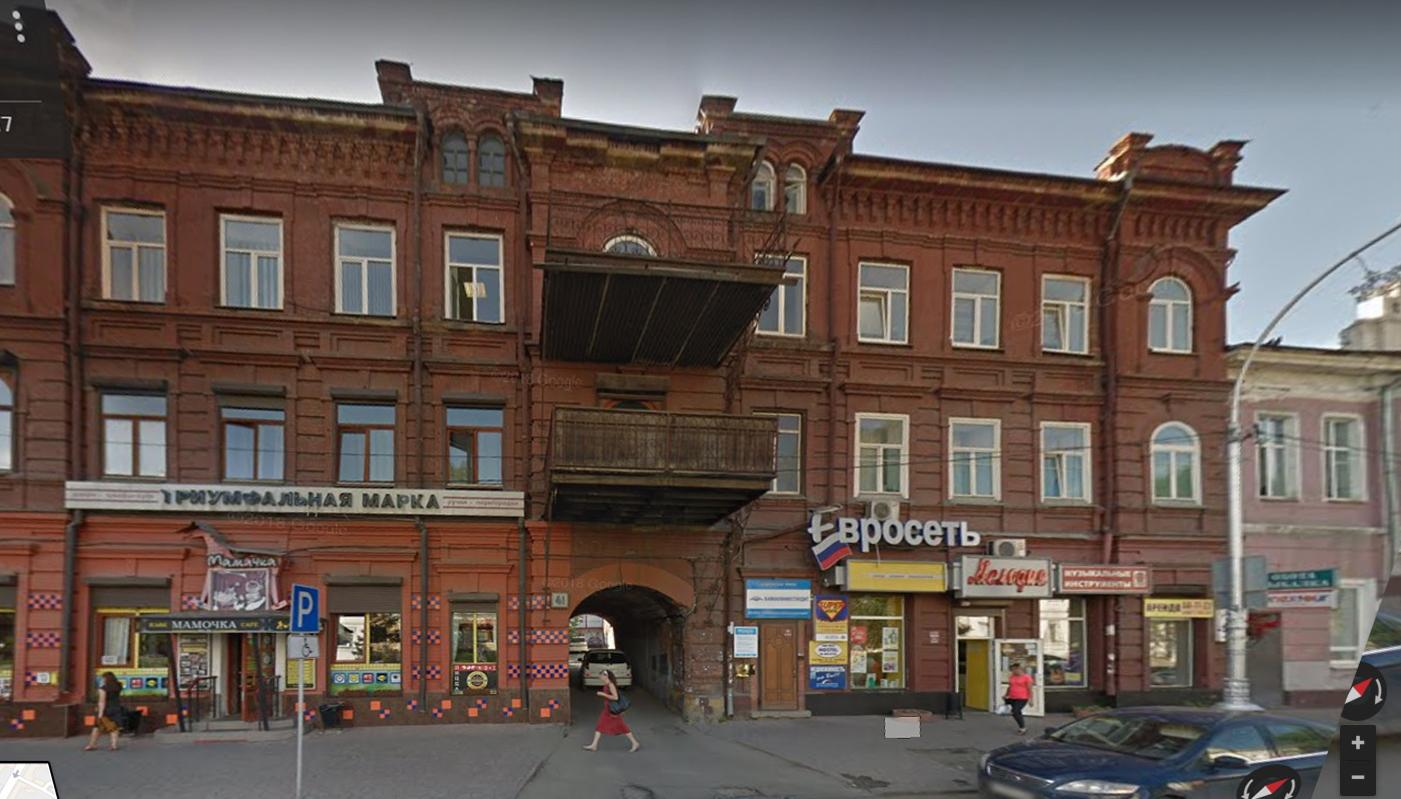
\includegraphics[width=7cm]{4} & 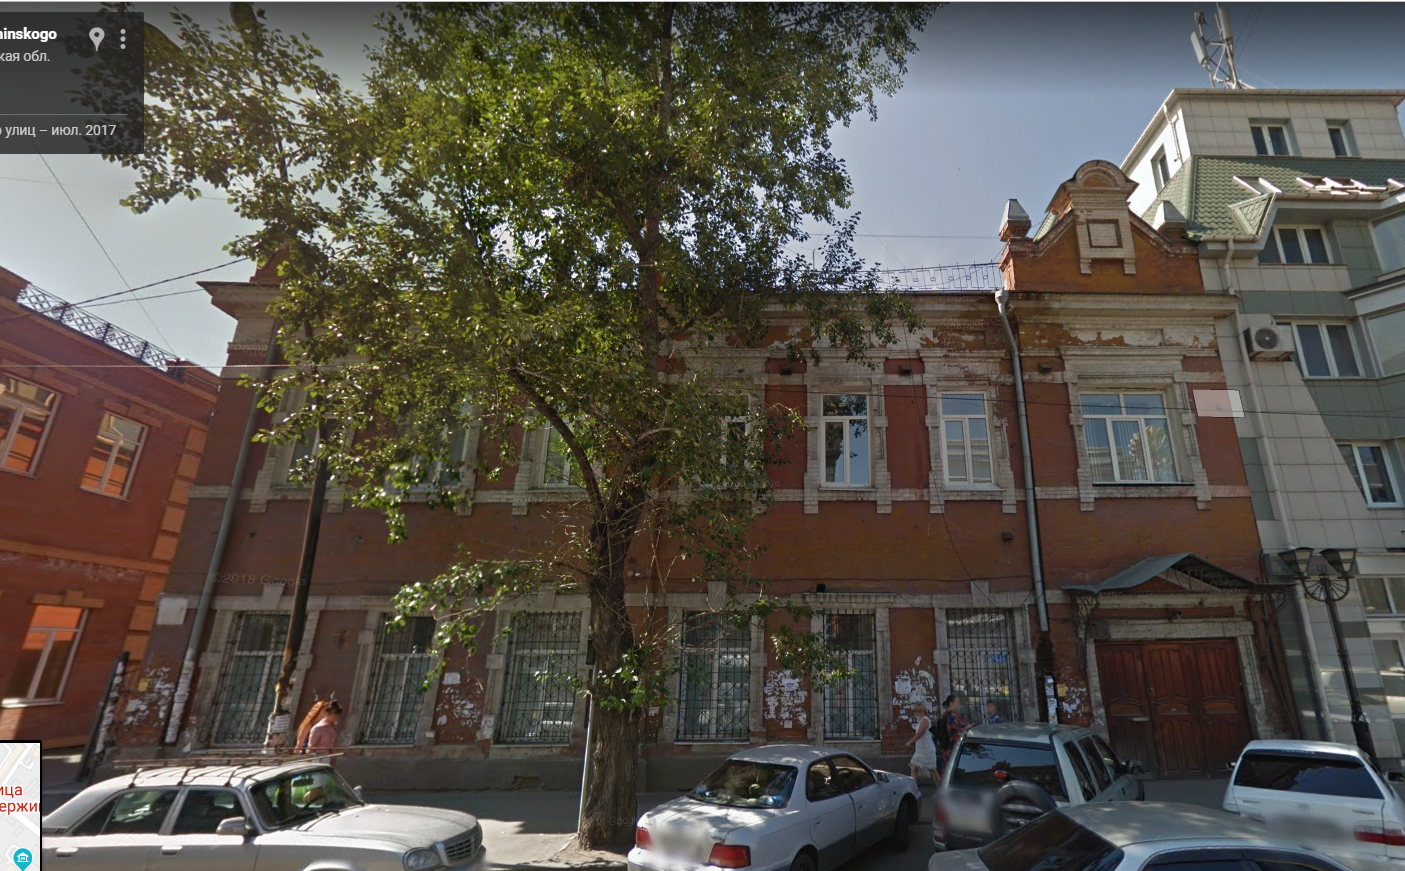
\includegraphics[width=6.5cm]{5} \\
    \hline
    Доходный дом Щербинина (Административное здание)

    Карла Маркса, 39 

    52.287527, 104.291251

    Ранее: Доходный дом с магазином Щербинина. & Усадьба Степанченкова 

    Дзержинского, 27 

    52.284905, 104.296066

    Ранее: Доходный дом  \\
    \hline
    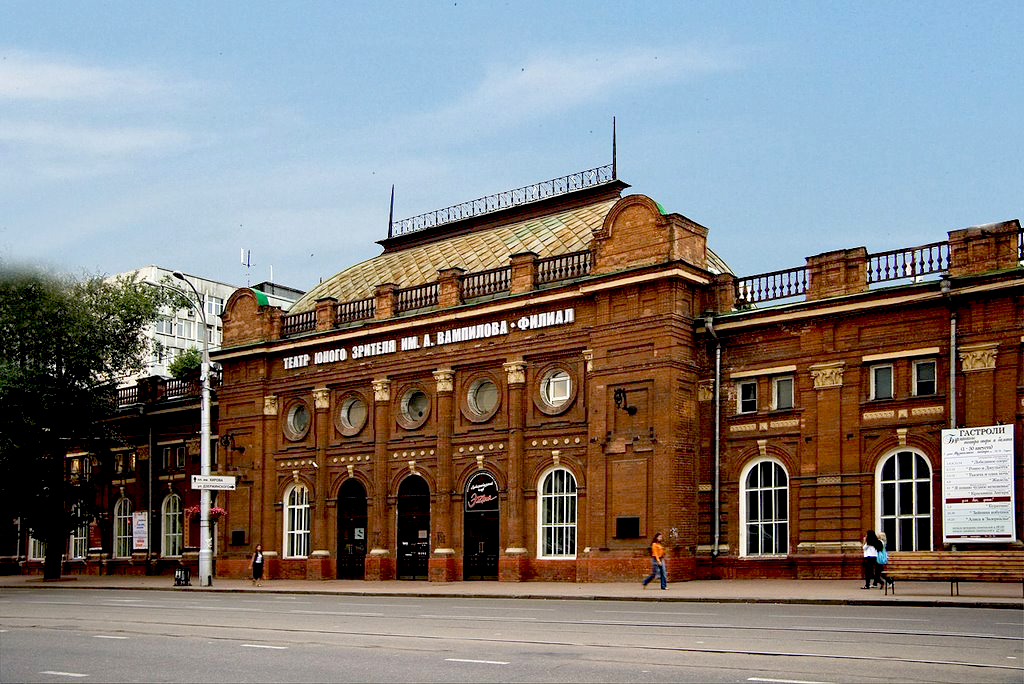
\includegraphics[width=7cm]{6} & 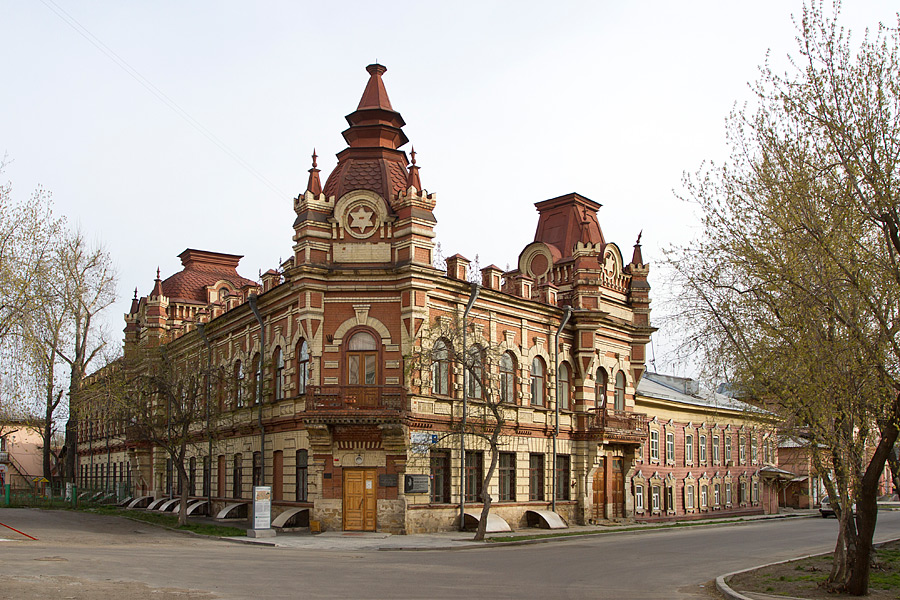
\includegraphics[width=7cm]{7} \\
    \hline
    Иркутская областная филармония 
    
    Дзержинского, 2 
    
    52.277985, 104.285367
    
    Ранее: ТРАМ (Театр рабочей молодежи) & Дом И.М. Файнберга  (отделы краеведения и библиографии, литературы по искусству и историко-культурного наследия областной библиотеки им. Молчанова-Сибирского)

    Халтурина, 1 

    52.289020, 104.286580

    Ранее: Доходный дом \\
    \hline
    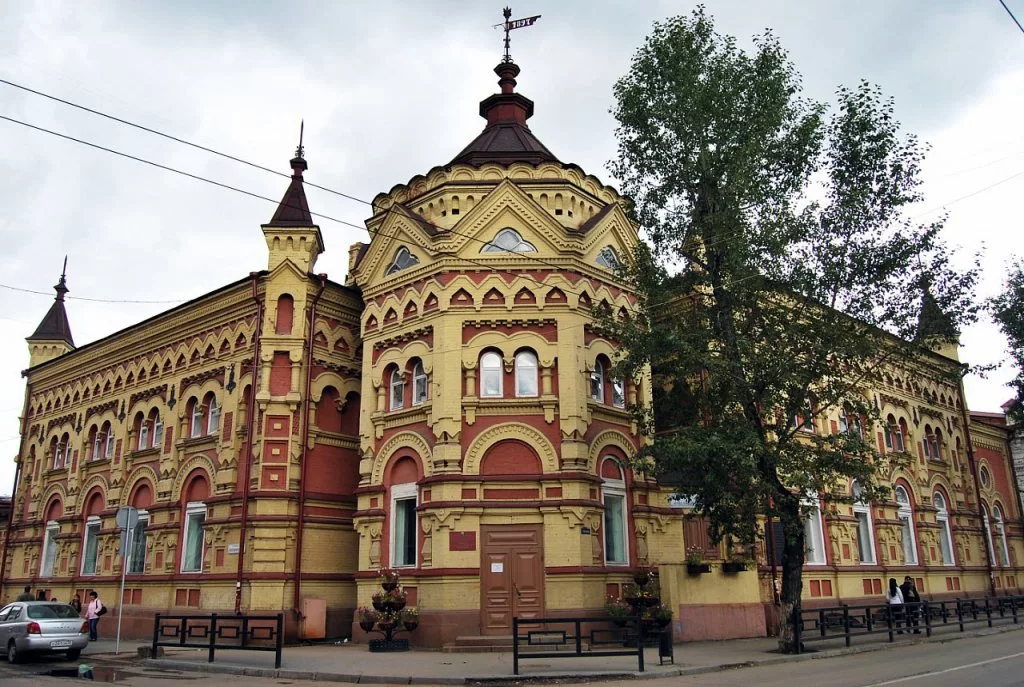
\includegraphics[width=7cm]{8} & 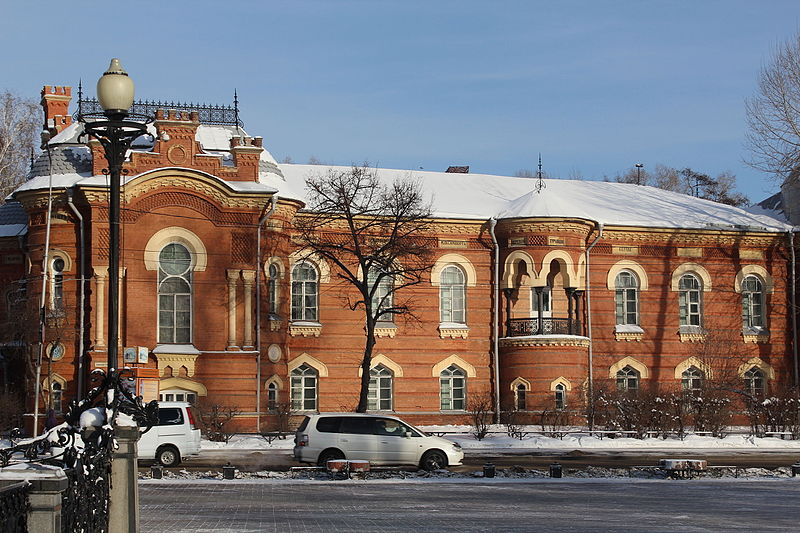
\includegraphics[width=7cm]{9} \\
    \hline
    Дворец детского и юношеского творчества 
    
    Желябова, 5 

    52.287770, 104.284846

    Ранее: особняк купца-миллионера А. Ф. Второва & Иркутский областной краеведческий музей 

    Карла Маркса, 13 
    
    52.281787, 104.284200 
    
    Ранее: сразу строился как Иркутский областной краеведческий музей \\
    \hline
    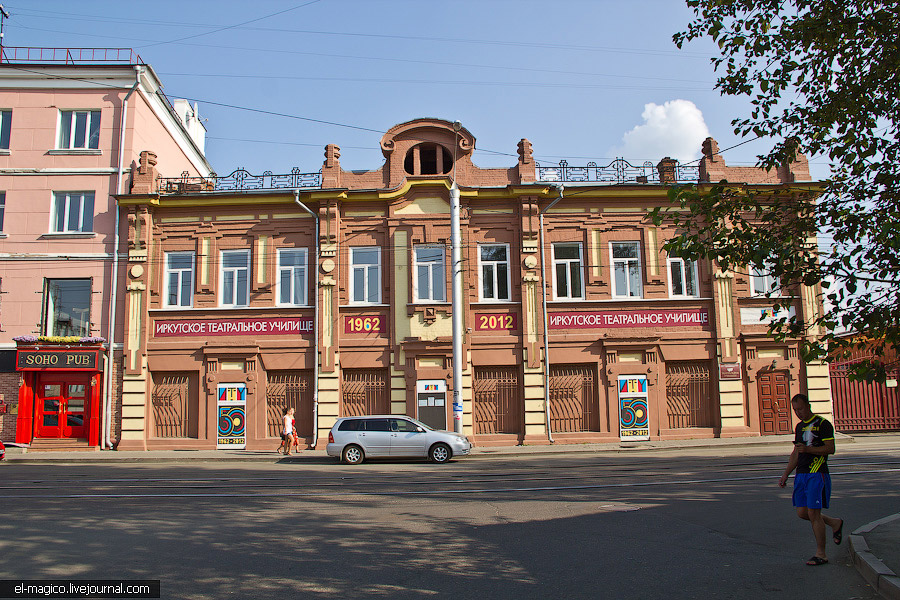
\includegraphics[width=7cm]{10} & 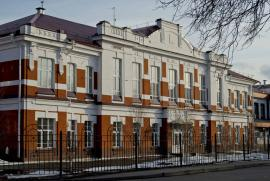
\includegraphics[width=7cm]{11} \\
    \hline
    Иркутское театральное училище
    
    Тимирязева, 20
    
    52.280564, 104.295456 

    Ранее: Дом-усадьбу Абрама Элоевича Кринкевича & Городского начальное училище им. Н.В. Гоголя (МБОУ г. Иркутска СОШ №11)
    
    Богданова переулок, 6 

    52.286112, 104.284532
    
    Ранее: сразу строилось как Городского начальное училище им. Н.В. Гоголя \\
    \hline    
\end{longtable}

\textit{Оценка - 5 баллов}

Составлен файл JSON, содержащий описание расположения объектов, соотношение количества клеток  разбиения фрагмента карты на поля: 12 клеток по высоте и 12 клеток по ширине (низкое разрешение), указание соответствия координат (х,у) гео-локационным координатам объектов при данном разбиении (разрешении): 

\inputminted[fontsize=\footnotesize, linenos]{json}{final/command_tour/ar/task_01/source.json}

При загрузке данного фрагмента  JSON валидатор (\url{https://jsonlint.com}) не выдает ошибок, а формат 
фрагмента совпадает с заданным шаблоном, рис.1.3.

\putImgWOCaption{16cm}{valid}

\begin{center}
    Рис.1.3. Результат работы  JSON валидатора (\url{https://jsonlint.com})
\end{center}

\markSection

Данное решение предоставляет 1 клеточную карту с JSON объектами. - \textit{1.7 баллов}. Полностью аналогично могут быть сформированы json файлы для высокого и среднего разрешения представления объектов на данной территории - \textit{+3.4 балла}. \textit{Общее количество баллов за полное выполнение этого пункта задания 5.1}.

Для каждой достопримечательности в файле указана широта и долгота - \textit{6.8 баллов}.

Для каждой достопримечательности правильно выбраны координаты на клеточном поле - \textit{5.1 баллов}.

Общее количество баллов за задачу 1 равно 35.